% !TeX spellcheck = ru_RU-Russian
\section{Технический проект}
\subsection{Общая характеристика организации решения задачи}

Необходимо спроектировать и разработать систему тестирования для контроля и оценки знаний.

Система тестирования представляет собой набор взаимосвязанных окон, содержащих текстовую и графическую информацию, которые сгруппированы по разделам. 

\subsection{Обоснование выбора технологии проектирования}

На сегодняшний день информационный рынок, поставляющий программные решения в выбранной сфере, предлагает множество продуктов, позволяющих достигнуть поставленной цели – разработки системы тестирования.

\subsubsection{Описание используемых технологий и языков программирования}

В процессе разработки системы тестирования используются программные средства и язык программирования. Каждое программное средство и язык программирования применяется для круга задач, при решении которых они необходимы.

\subsubsection{Язык программирования Python}

Python — это язык программирования, который широко используется в интернет-приложениях, разработке программного обеспечения, науке о данных и машинном обучении (ML). Разработчики используют Python, потому что он эффективен, прост в изучении и работает на разных платформах.

\subsubsection{Библиотека Tkinter}
Tkinter — это кроссплатформенный графический интерфейс Python, позволяющий работать с библиотекой Tk. Он содержит элементы графического интерфейса пользователя (GUI — Graphical User Interface), с помощью которых можно создавать различные приложения.

\subsubsection{Достоинства языка Python}

К плюсам Python относятся: Простота. Его часто советуют в качестве первого “базового” языка, так как он очень прост в изучении и исполнении. В процессе написания программы не требуется использование фигурных скобок, как в других языках, что позволяет не отвлекаться на переключение между клавишами уделять больше внимания разработке программы. Обширность применения.

\subsubsection{Недостатки языка Python}

Низкая скорость выполнения (причины: интерпретация, динамическая типизация) по сравнению с Delphi, C/C++, C\#, Java.
Отсутствие библиотек для создания "родных" интерфейсов для Windows.

\subsubsection{Описание формата хранения вопросов}

Для хранения данных вопросов был выбран язык разметки JSON (JavaScript Object Notation), так как он хорошо подходит для обмена данными между различными системами и приложениями благодаря своей легкости и удобству чтения.

Общая структура хранения вопросов теста:
\begin{itemize}
	\item корневой элемент - JSON-объект, содержащий информацию о составе теста;
	\item "<test\_name"> - строковое поле, представляющее название теста;
	\item "<questions"> - массив JSON-объектов, каждый из которых описывает один вопрос теста.
\end{itemize}

В структуре хранения вопроса используется целое число -- перечисление "<QuestionType">, оно позволяет однозначно определить тип вопроса и правильно интерпретировать данные, содержащиеся в массиве ответов, делает формат хранения вопросов более структурированным и понятным. Подробное описание перечисления представлено в структуре хранения вопроса.

Структура хранения вопроса:
\begin{itemize}
	\item "<type"> - целое число, определяющее тип вопроса. Значение этого поля соответствует одному из значений перечисления: 0 (или QuestionType.base)- вопрос с текстовым вводом ответа, 1 (или QuestionType.radio\_button): Вопрос с выбором одного правильного ответа из нескольких предложенных вариантов, 2 (или QuestionType.check\_button): Вопрос с выбором нескольких правильных ответов из нескольких предложенных вариантов;
	\item "<text"> - строковое поле, содержащее текст вопроса;
	\item "<answers"> - массив JSON-объектов, каждый из которых описывает варианты ответов на вопрос. Структура "<answers"> зависит от типа вопроса.
\end{itemize}

Структура хранения ответа:
\begin{itemize}
	\item "<text"> - строковое поле, содержащее текст ответа;
	\item "<is\_correct"> - логическое значение (true или false), указывающее, является ли данный ответ правильным.
\end{itemize}

На рисунке ~\ref{question_storage_format:image} приведён пример хранения вопросов теста по описанному формату.

\begin{figure}[H]
	\centering
	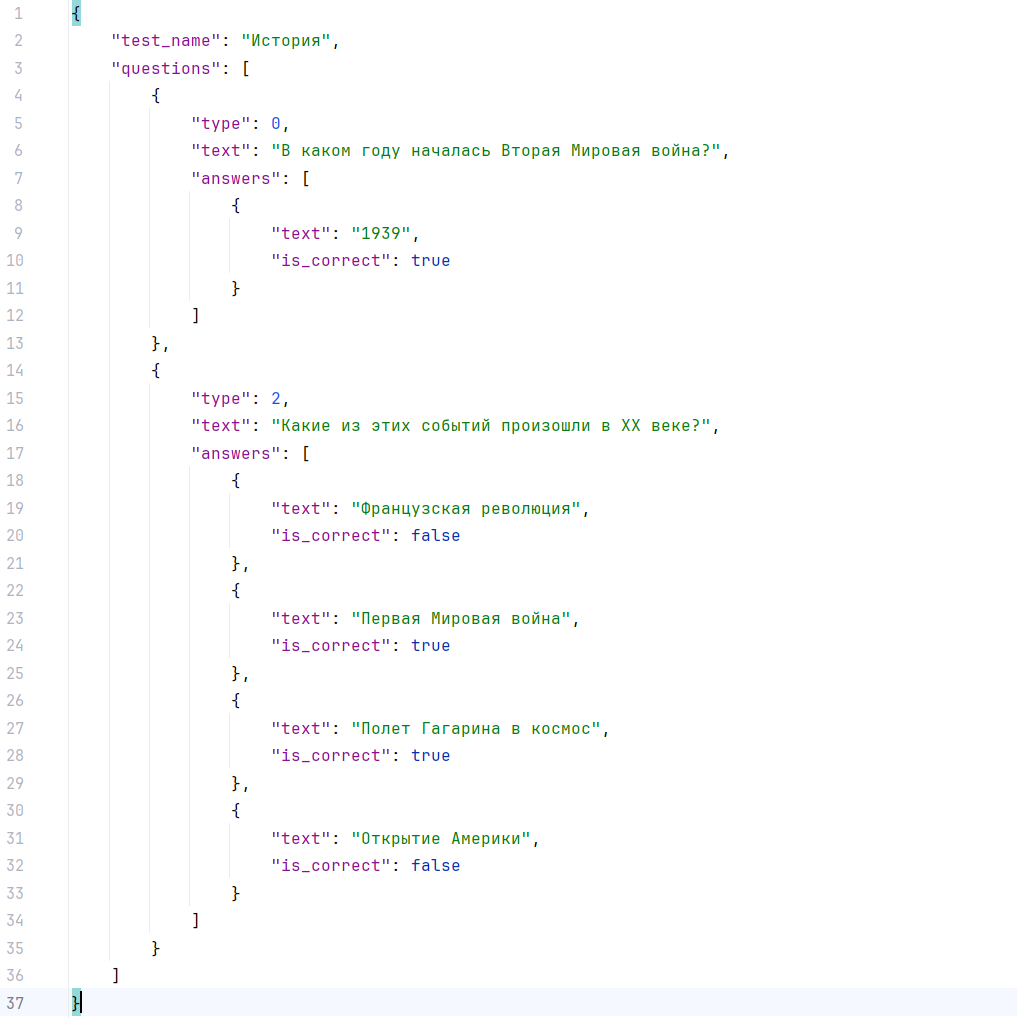
\includegraphics[width=1\linewidth]{формат_хранения_теста.png}
	\caption{Пример хранения вопросов теста с помощью JSON}
	\label{question_storage_format:image}
\end{figure}

\subsection{Диаграмма компонентов и диаграмма классов}

Диаграмма компонентов описывает особенности физического представления разрабатываемой системы. Она позволяет определить архитектуру системы, установив зависимости между программными компонентами, в роли которых может выступать как исходный, так и исполняемый код. Основными графическими элементами диаграммы компонентов являются компоненты, интерфейсы, а также зависимости между ними. На рисунке \ref{system_template:image} изображена диаграмма компонентов для проектируемой системы. Она включает в себя основные модули приложения. 

\newpage

\begin{landscape}
	\begin{figure}[ht]
		\center{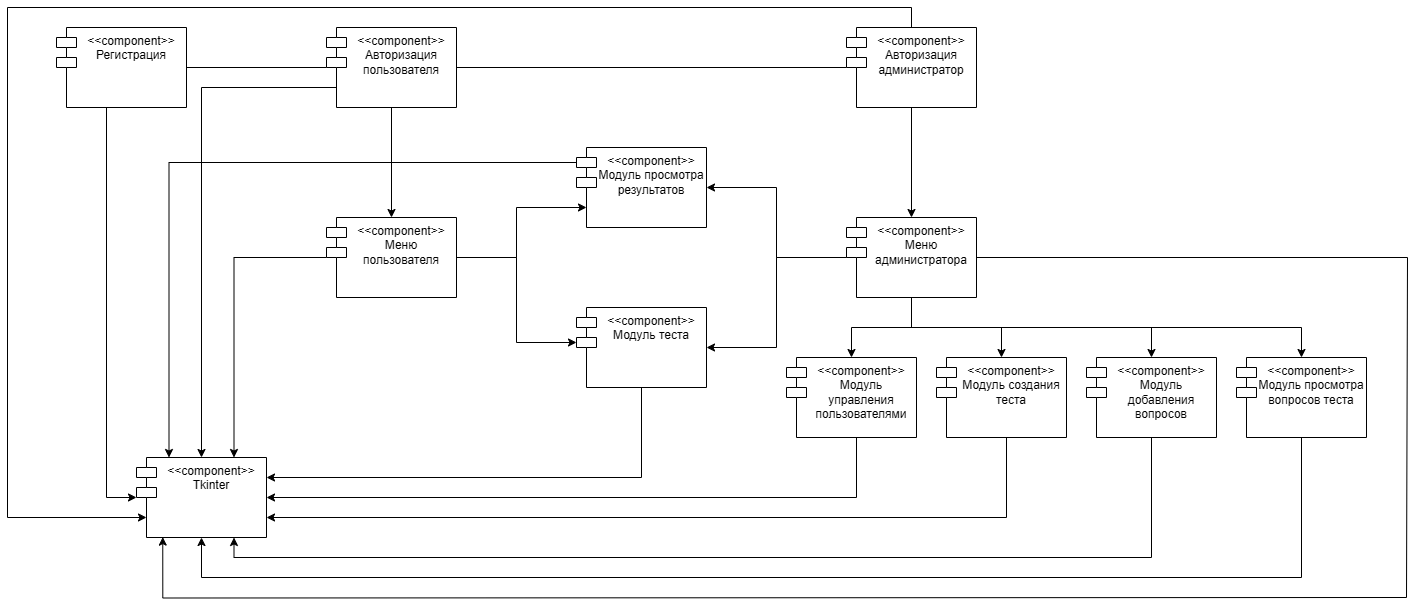
\includegraphics[width=1\linewidth]{диаграмма_компонентов.png}}
		\caption{Диаграмма компонентов}
		\label{system_template:image}
	\end{figure}
\end{landscape}

Любой компонент должен быть вызван в сценарии окна системы тестирования. Окно передает данные компоненту в момент вызова последнего.

При вызове компонента в сценарии системы тестирования указывается значения имя пользователя и набор вопросов соответствующий выбранному тесту, которые далее посредством ссылок на объекты классов, описывающих данную информацию передаются в следующее окно.

В зависимости от типа вопроса инициализируется соответствующее отображение с вариантами ответа.

Работа компонента заканчивается в момент закрытия главного окна.

На рисунке \ref{class_diagram:image} представлена диаграмма классов.

\newpage
\begin{landscape}
	\begin{figure}[ht]
		\center{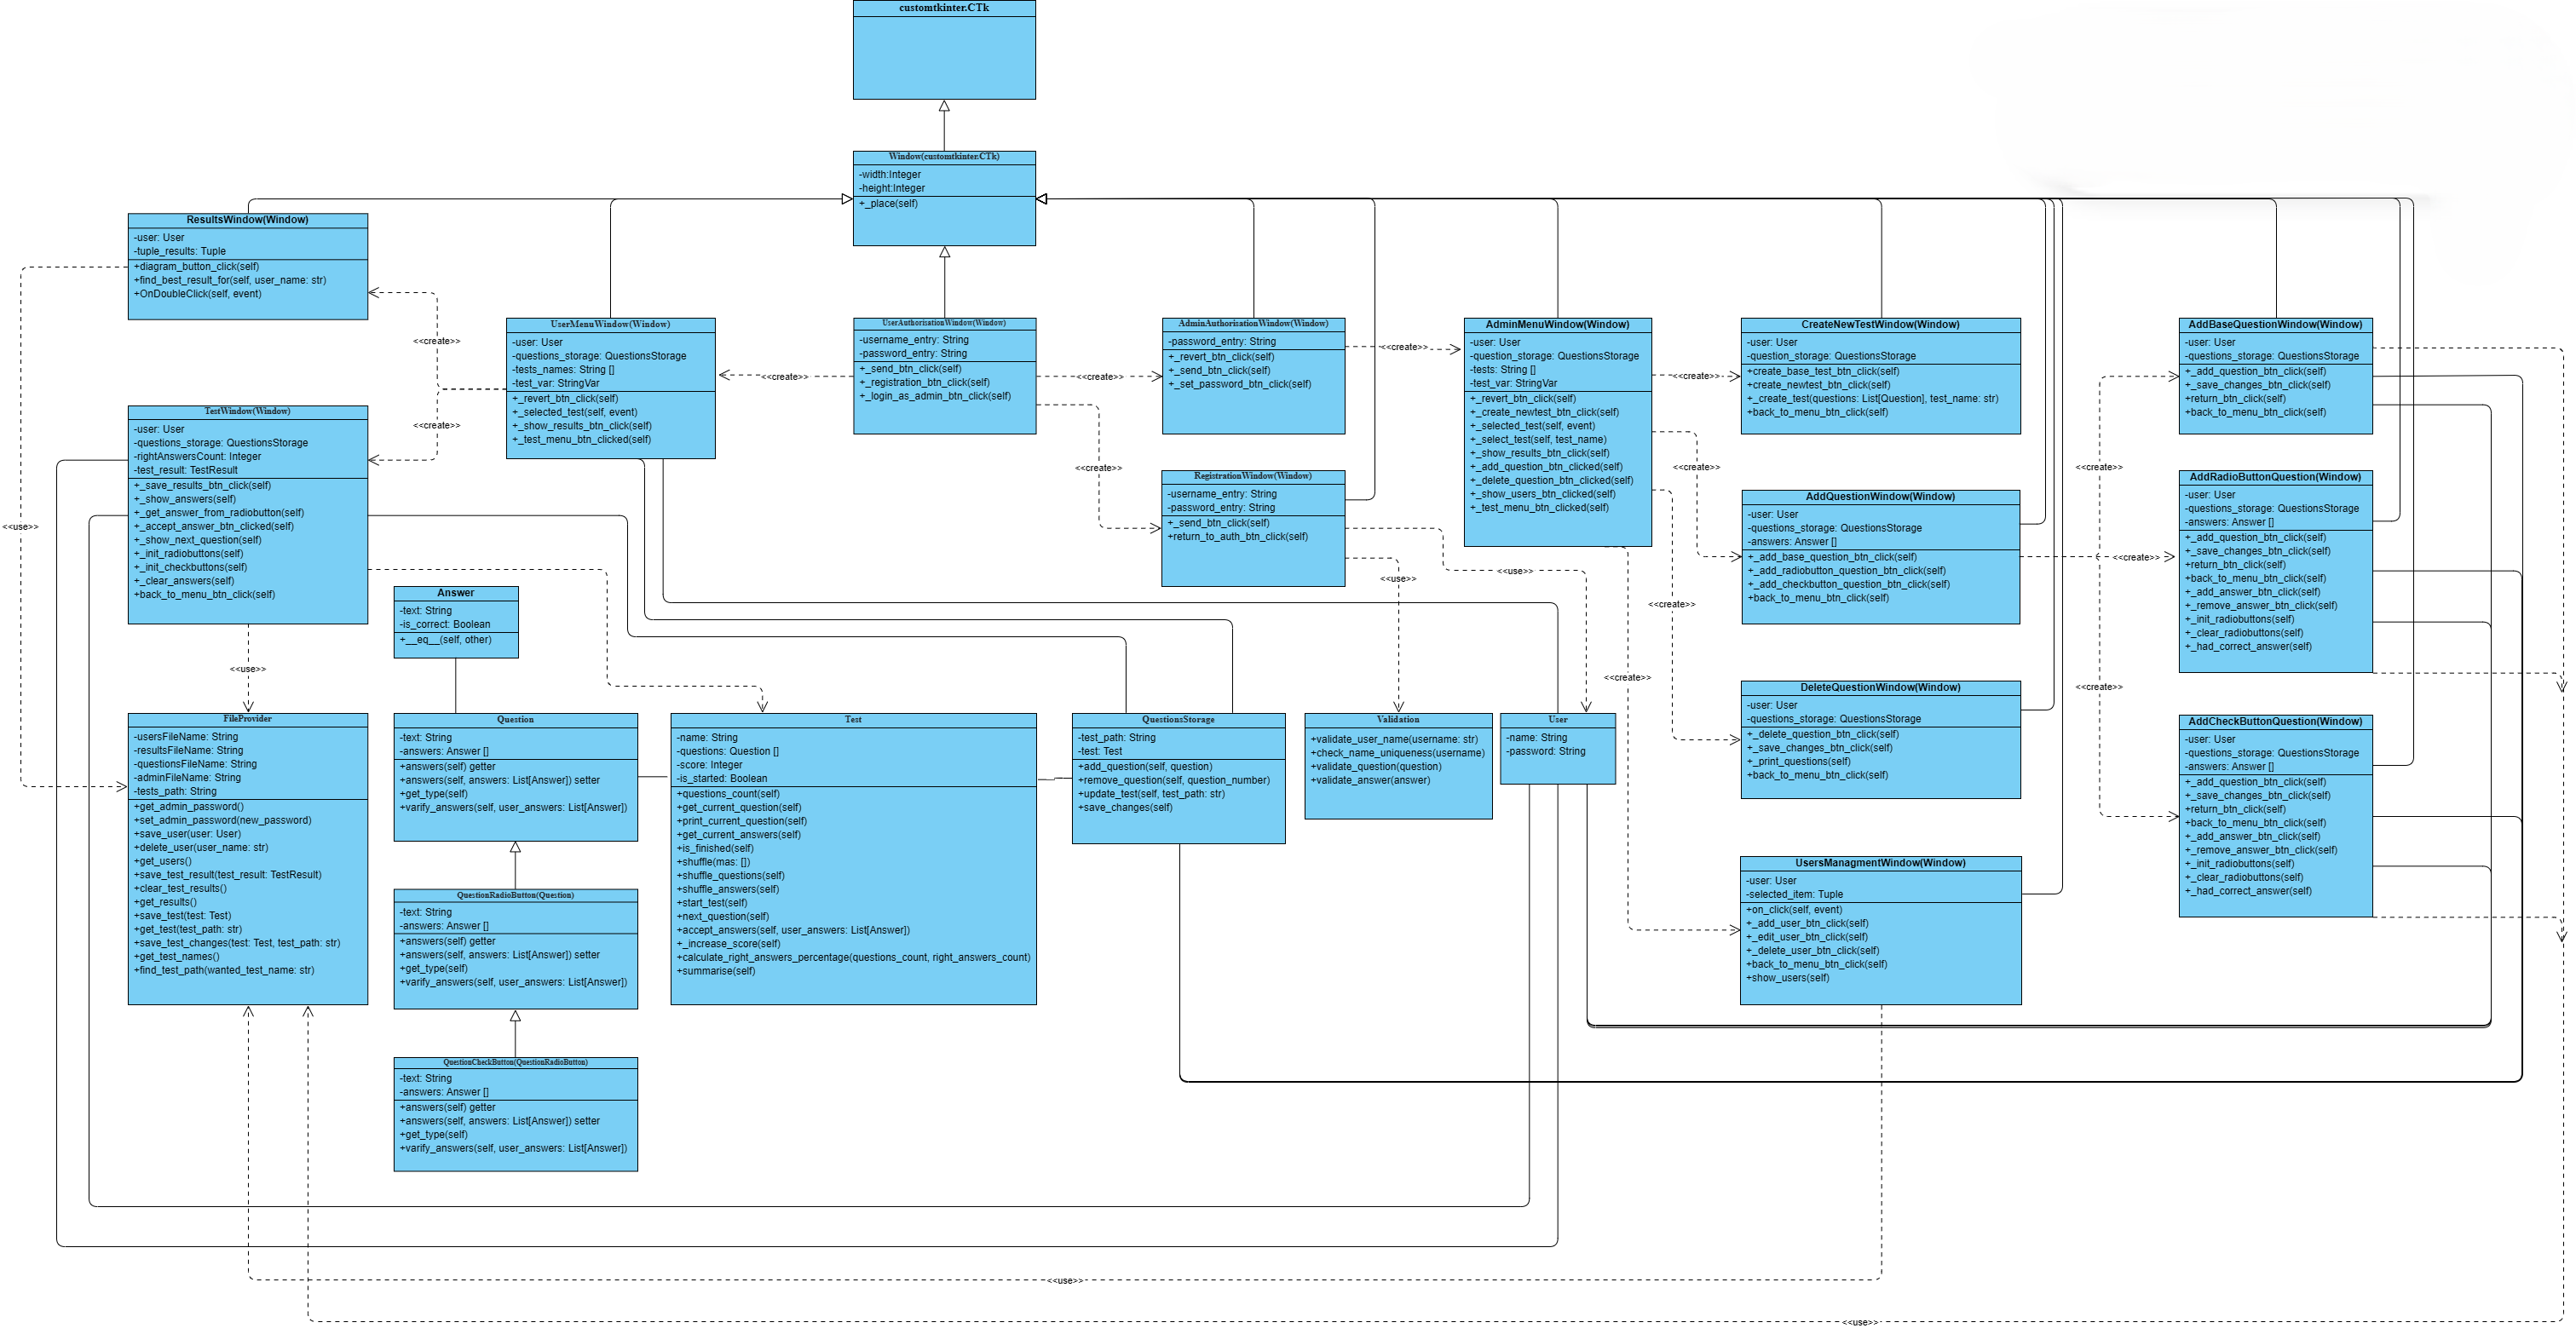
\includegraphics[width=1\linewidth]{диаграмма_классов.png}}
		\caption{Диаграмма классов}
		\label{class_diagram:image}
	\end{figure}
\end{landscape}

\newpage

\subsection{Содержание информационных блоков. Основные классы}

Проанализировав требования, можно выделить пять основных классов:
\begin{enumerate}
	\item "<Пользователь">.
	\item "<Вопрос">.
	\item "<Ответ">.
	\item "<Тест">.
	\item "<Результат">.
\end{enumerate}

В состав сущности "<Пользователь"> можно включить атрибуты, представленные в таблице \ref{user:table}.

\begin{xltabular}{\textwidth}{|l|l|p{1.7cm}|X|}
	\caption{Атрибуты класса "<Пользователь">\label{user:table}}\\ \hline
	\centrow Поле & \centrow Тип & \centrow Обяза\-тельное & \centrow Описание \\ \hline
	\thead{1} & \thead{2} & \centrow 3 & \centrow 4 \\ \hline
	\endfirsthead
	\thead{1} & \thead{2} & \centrow 3 & \centrow 4 \\ \hline
	\finishhead
	\ name & String & true & Имя пользователя
\end{xltabular}

В состав класса "<Вопрос"> можно включить атрибуты, представленные в таблице \ref{question:table}.

\begin{xltabular}{\textwidth}{|l|l|p{1.7cm}|X|}
	\caption{Атрибуты класса "<Вопрос">\label{question:table}}\\ \hline
	\centrow Поле & \centrow Тип & \centrow Обяза\-тельное & \centrow Описание \\ \hline
	\thead{1} & \thead{2} & \centrow 3 & \centrow 4 \\ \hline
	\endfirsthead
	\thead{1} & \thead{2} & \centrow 3 & \centrow 4 \\ \hline
	\finishhead
	\ text & String & true & Текст вопроса \\ \hline
	answers & List[Answer] & true & Список вопросов
\end{xltabular}

В состав класса "<Ответ"> можно включить атрибуты, представленные в таблице \ref{answer:table}.

\begin{xltabular}{\textwidth}{|l|l|p{1.7cm}|X|}
	\caption{Атрибуты класса "<Ответ">\label{answer:table}}\\ \hline
	\centrow Поле & \centrow Тип & \centrow Обяза\-тельное & \centrow Описание \\ \hline
	\thead{1} & \thead{2} & \centrow 3 & \centrow 4 \\ \hline
	\endfirsthead
	\thead{1} & \thead{2} & \centrow 3 & \centrow 4 \\ \hline
	\finishhead
	\ text & String & true & Текст ответа \\ \hline
	is correct & Bool & false & Корректность вопроса
\end{xltabular}

В состав класса "<Тест"> можно включить атрибуты, представленные в таблице \ref{test:table}.

\begin{xltabular}{\textwidth}{|l|l|p{1.7cm}|X|}
	\caption{Атрибуты класса "<Тест">\label{test:table}}\\ \hline
	\centrow Поле & \centrow Тип & \centrow Обяза\-тельное & \centrow Описание \\ \hline
	\thead{1} & \thead{2} & \centrow 3 & \centrow 4 \\ \hline
	\endfirsthead
	\thead{1} & \thead{2} & \centrow 3 & \centrow 4 \\ \hline
	\finishhead
	\ name & String & true & имя теста \\ \hline
	questions & List[Question] & true & Список вопросов \\ \hline
	score & Integer & false & Счёт \\ \hline
	is started & Bool & false & Состояние теста \\ \hline
	current question id & Integer & false & ID текущего вопроса \\ \hline
	current answers & List[Answer] & false & Список ответов текущего вопроса
\end{xltabular}

В состав класса "<Результат"> можно включить атрибуты, представленные в таблице \ref{result:table}.

\begin{xltabular}{\textwidth}{|l|l|p{1.7cm}|X|}
	\caption{Атрибуты класса "<Результат">\label{result:table}}\\ \hline
	\centrow Поле & \centrow Тип & \centrow Обяза\-тельное & \centrow Описание \\ \hline
	\thead{1} & \thead{2} & \centrow 3 & \centrow 4 \\ \hline
	\endfirsthead
	\thead{1} & \thead{2} & \centrow 3 & \centrow 4 \\ \hline
	\finishhead
	\ user & User & true & Пользователь \\ \hline
	right answers count & Integer & true & Количество правильных ответов \\ \hline
	completion time & datetime & false & Время завершения теста
\end{xltabular}

В системе предусмотрен внутренний механизм связи между разделами и элементами информационных блоков, поэтому введения дополнительных идентификаторов при реализации связей между сущностями не предполагается.

Экземпляры сущностей реализуются в информационных блоках посредством элементов, атрибуты сущности – посредством полей и свойств элемента. 

\subsection{Проектирование пользовательского интерфейса}

На основании требований к пользовательскому интерфейсу, представленных в пункте 2.6 технического задания, был разработан графический интерфейс десктопного приложения. Для создания пользовательского
интерфейса используется библиотека Custom Tkinter.
На рисунке ~\ref{user_auth:image} представлен макет интерфейса вкладки «Авторизация пользователя». Макет содержит следующие элементы:
\begin{enumerate}
	\item Текстовое поле для ввода имени пользователя.
	\item Текстовое поле для ввода пароля пользователя.
	\item Кнопка авторизации, проверяет введённые данные пользователя, если они верны открывает меню пользователя.
	\item Кнопка регистрации, открывает окно регистрации пользователя.
	\item Кнопка для авторизации администратора. 
\end{enumerate}

\begin{figure}[H]
	\center{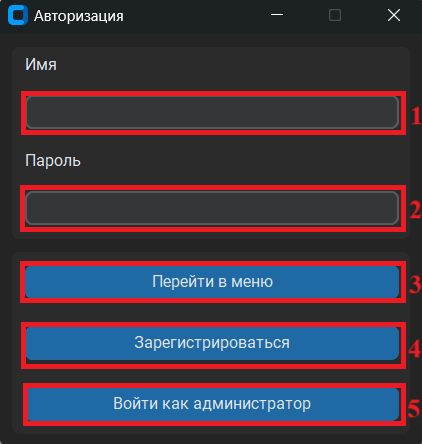
\includegraphics[width=0.6\linewidth]{макет_авторизация_пользователя}}
	\caption{Макет авторизации пользователя}
	\label{user_auth:image}
\end{figure}

На рисунке ~\ref{admin_auth:image} представлен макет интерфейса вкладки «Авторизация администратора». Макет содержит следующие элементы:
\begin{enumerate}
	\item Текстовое неизменяемое поле с надписью "Администратор".
	\item Текстовое поле для ввода пароля администратора.
	\item Кнопка авторизации, проверяет введённые данные пользователя, если они верны открывает меню администратора.
	\item Кнопка смены пароля администратора.
	\item Кнопка для авторизации пользователя. 
\end{enumerate}

\begin{figure}[H]
	\center{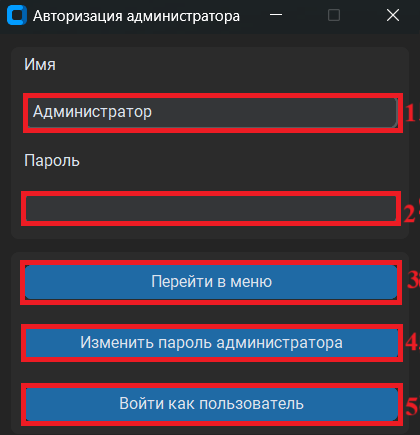
\includegraphics[width=0.6\linewidth]{макет_авторизация_админ}}
	\caption{Макет авторизации администратора}
	\label{admin_auth:image}
\end{figure}

На рисунке ~\ref{user_menu:image} представлен макет интерфейса вкладки «Меню пользователя». Макет содержит следующие элементы:
\begin{enumerate}
	\item Выпадающий список тестов для выбора.
	\item Кнопка запуска теста.
	\item Кнопка перехода к окну результатов пройденных тестов.
	\item Кнопка возврата к авторизации.
\end{enumerate}

\begin{figure}[H]
	\center{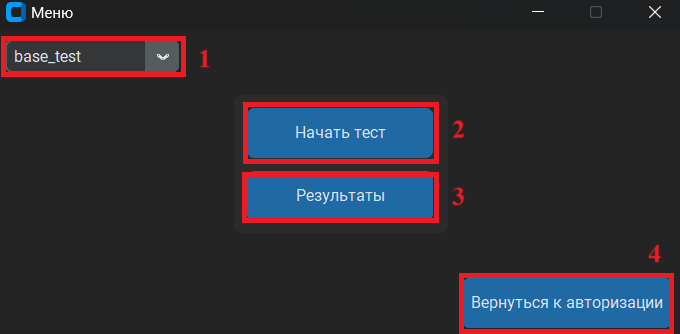
\includegraphics[width=1\linewidth]{макет_меню_пользователя}}
	\caption{Макет меню пользователя}
	\label{user_menu:image}
\end{figure}

На рисунке ~\ref{admin_menu:image} представлен макет интерфейса вкладки «Меню администратора». Макет содержит следующие элементы:
\begin{enumerate}
	\item Выпадающий список тестов для выбора.
	\item Кнопка создания нового теста.
	\item Кнопка добавления нового вопроса в выбранный тест.
	\item Кнопка перехода к окну со списком вопросов теста.
	\item Кнопка запуска теста.
	\item Кнопка просмотра результатов всех пользователей.
	\item Кнопка перехода в окно управления пользователями.
	\item Кнопка возврата к окну авторизации.
\end{enumerate}

\begin{figure}[H]
	\center{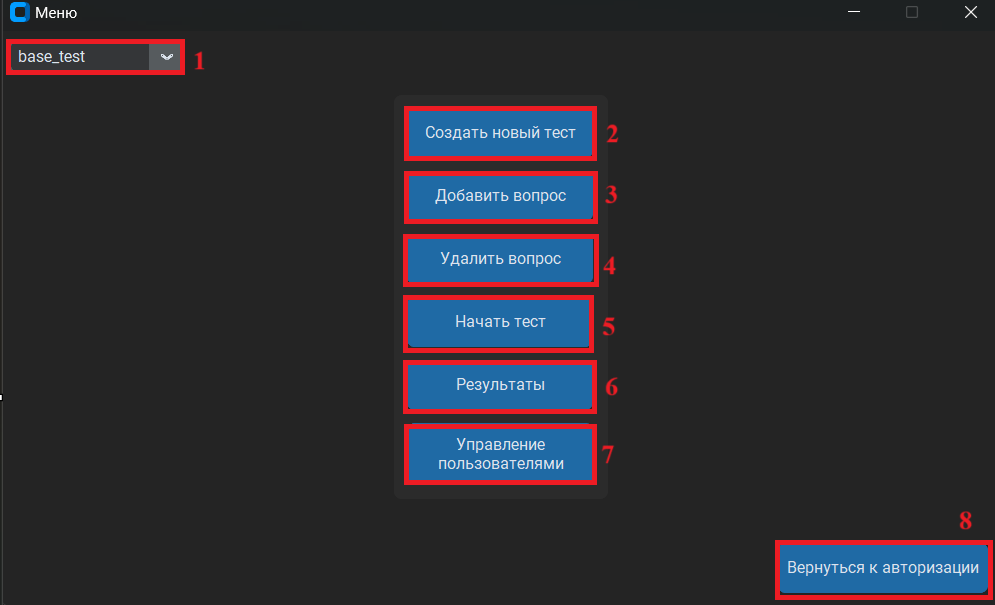
\includegraphics[width=1\linewidth]{макет_меню_админ}}
	\caption{Макет меню администратора}
	\label{admin_menu:image}
\end{figure}
